\section{Exact Model}
\label{sec:exact}

Fig.~\ref{fig:overview} gives an overview of how the exact model is used. It computes the reference policies, tunes the rules, scores every trained agent, and gives the expected return that is used to choose hyperparameters.

\begin{figure*}[t]
\centering
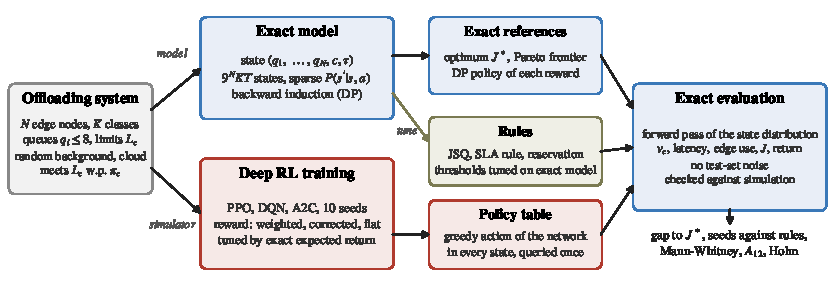
\includegraphics[width=\textwidth]{fig_overview.pdf}
\caption{Overview of the evaluation method. The exact model of each system gives the optimum, the Pareto frontier and the DP policy of each reward, and tunes the rules. Agents learn in the simulator only. Each trained network is turned into a table over all states and scored by the same exact forward pass as the rules and the DP policies.}
\label{fig:overview}
\end{figure*}

\subsection{The Observation Is the State}
In the nominal system the background schedule depends only on the step $t$, which the time share $\tau_t$ gives exactly. In the larger systems the background arrivals of each step are drawn independently of the past. In both cases the only random parts of a step are the service events, the background arrivals, the cloud outcome and the class of the next task, and all of them are independent of the history given the current queues and step. The observation $s_t$ is therefore a full description of the state, and each system is a finite-horizon Markov decision process \cite{puterman1994}. By the standard result for such processes, a deterministic policy that depends only on $s_t$ is optimal among all policies, including those that use the full history \cite{puterman1994}.

\subsection{Size and Transitions}
There are $9^N$ queue states, $K$ classes and $T=200$ steps, which gives the state counts of Table~\ref{tab:systems}. For a queue state and an action, the next queue state follows from three parts. The placed task joins its queue up to the cap of 8. The background tasks of the step join the shortest queue, with ties going to the lowest node index as in the simulator. Each non-empty queue then loses one task with probability $d_i$, independently of the others. This gives at most $2^N$ next queue states for each number of background tasks. The transitions are stored as one sparse matrix for each action and are built once. The class of the next task is drawn independently with probabilities $p_c$.

\subsection{Optimal Policies by DP}
Let $g(s,a)$ be the expected cost of action $a$ in state $s$, and let $P(s' \mid s,a)$ be the transition probability. Backward induction computes
\begin{equation}
V_t(s) = \min_{a} \Big[ g(s,a) + \sum_{s'} P(s' \mid s, a)\, V_{t+1}(s') \Big],
\label{eq:bellman}
\end{equation}
with $V_T = 0$, and the minimizing action gives the optimal policy at each step \cite{puterman1994}. With $g$ equal to $e_c$ times the chance of a miss, the expected total cost over an episode is $T$ times $J$, because the expected number of tasks of each class does not depend on the policy. The result is the policy with the lowest possible SLA cost, called the optimum. With $g = -\mathbb{E}[R_t]$ from Eq.~\eqref{eq:reward}, the result is the policy that a perfect learner of that reward would find, called the DP policy of the reward.

\subsection{Pareto Frontier}
For two classes, the paper solves Eq.~\eqref{eq:bellman} with $g$ equal to $\mu/p_1$ for a missed critical task and $(1-\mu)/p_2$ for a missed analytics task, for 101 values of $\mu$ between 0 and 1. Each solution minimizes $\mu\, v_1 + (1-\mu)\, v_2$. The resulting pairs of miss rates trace the lower boundary of all reachable pairs.

\subsection{Exact Evaluation of Any Policy}
For a deterministic policy given as a table over all states, the exact model starts from empty queues and propagates the probability of each state forward through the 200 steps. At each step it adds the expected misses, latency and edge placements of each class. Dividing by the expected number of tasks of each class gives the exact $v_c$, mean latencies, edge use and $J$. These are the values that a simulation with infinitely many episodes would give. A trained neural network is turned into such a table by asking it for its greedy action in every state once. The time share $\tau_t$ is computed with the same 32-bit numbers as in the simulator, so the table gives exactly the action that the network gives during a simulation. The same forward pass gives the exact expected return of a policy under any reward, which is used for hyperparameter selection in Section~\ref{sec:method}.

\subsection{Checks Against the Simulator}
The open test suite checks the exact model against the simulator. With the nominal parameters, the general simulator produces the same observations and rewards as the simulator of the conference version for 1,000 steps, and the general model gives the same optimal SLA cost as the earlier two-node model to within $10^{-12}$. In Hetero3 and Hetero3-3C, exact and simulated miss rates agree within one percentage point over 400 episodes for the optimum, and within 1.5 points for a random policy table, which is about three standard errors. Every transition matrix row sums to one, the optimum is never above any rule, and the exact expected return of a DP policy agrees with a 300-episode simulation within three standard errors.

\subsection{Cost of the Exact Solution}
Table~\ref{tab:scaling} shows how the exact solution grows with the number of edge nodes, for a homogeneous system with two classes at load 1 on one CPU core. Each extra node multiplies the queue states by 9 and the stored transitions by 14 to 24. Five nodes give 23.6 million states and need 16\,s to solve and 26\,s for one exact evaluation. A sixth node would again multiply the stored transitions by about 14, to roughly $1.6\times10^8$, which needs several gigabytes of memory. The exact benchmark is therefore a tool for systems of up to four or five nodes. A learned policy has a fixed size and decision time, whatever the number of nodes.

\begin{table}[t]
\caption{Size and time of the exact DP for $N$ equal edge nodes, two classes and load 1 (one CPU core).}
\label{tab:scaling}
\centering
\footnotesize
\setlength{\tabcolsep}{3pt}
\begin{tabular}{@{}rrrrrr@{}}
\toprule
$N$ & States & Transitions & Solve (s) & Evaluate (s) & Memory (MB) \\
\midrule
SCALINGROWS
\bottomrule
\end{tabular}
\end{table}

\section{What Each Reward Optimizes}
\label{sec:reward}

\subsection{A Bonus Shifts Every Penalty}
The reward of Eq.~\eqref{eq:reward} gives $\beta$ for a met limit and $-w_c$ for a miss. Writing the reward of a missed task as $\beta - (w_c + \beta)$ shows that a miss costs $w_c + \beta$ relative to a met limit. This gives the following result.

\emph{Proposition 1.} For any policy, the expected total reward of an episode is
\begin{equation}
\mathbb{E}\Big[\sum_{t} R_t\Big] = T\beta - T\sum_c p_c\,(w_c + \beta)\, v_c - \kappa\, n_\text{cloud},
\label{eq:prop}
\end{equation}
where $n_\text{cloud}$ is the expected number of cloud placements. A policy maximizes the expected reward exactly when it minimizes $\sum_c p_c (w_c + \beta) v_c + \kappa\, n_\text{cloud}/T$.

\emph{Proof.} Each task gives $\beta - (w_{c_t} + \beta)\, m_t - \kappa\,\mathbf{1}[a_t=\text{cloud}]$. The expected number of tasks of class $c$ in an episode is $T p_c$ for every policy, because classes are drawn independently of the actions. The expected number of misses of class $c$ is therefore $T p_c v_c$, by the definition of $v_c$. Summing over the steps and taking expectations gives Eq.~\eqref{eq:prop}. The first term does not depend on the policy. \hfill$\blacksquare$

Three consequences follow. First, a learner of the weighted reward ranks misses by $w_c + \beta$, not by $w_c$. In the nominal system the penalties 10 and 2 act as 11 and 3, a ratio of 3.7 instead of the operator's 5. Second, the flat reward ranks all misses equally, so its optimal policy minimizes the overall miss rate plus the cloud term, whatever the operator weights are. Third, choosing
\begin{equation}
w_c = \alpha\, e_c - \beta, \qquad \alpha = \frac{\bar w + \beta}{\sum_c p_c e_c},
\label{eq:corrected}
\end{equation}
makes $w_c + \beta$ proportional to $e_c$ and keeps the average penalty at $\bar w$. This corrected reward ranks policies exactly as $J$ does, apart from the small cloud term. In the nominal system it gives penalties of 10.67 and 1.33. In the three-class systems it gives 11.17, 3.87 and 0.22, against weighted penalties of 10, 4 and 1. Proposition 1 holds for the undiscounted total reward. The learners of this paper use a discount factor below one, which the next subsection takes into account.

\subsection{Exact Consequences}
Table~\ref{tab:dprewards} gives the DP policy of each reward in each system. In the nominal system the weighted reward reaches an SLA cost of 0.2641, 1.0\% above the optimum of 0.2614, and the corrected reward reaches the optimum exactly. In Hetero3-3C the bonus moves the weighted reward 10.4\% above the optimum, while the corrected reward again reaches it. The flat reward is 65\% to 118\% above the optimum in every system. With a discount factor of 0.99, as used by the learners, the corrected reward stays within 0.8\% of the optimum in the first three systems and 4.1\% in Large4-3C. The flat reward gets worse with discounting in the larger systems, up to 174\% above the optimum.

\begin{table}[t]
\caption{Exact SLA cost of the optimum, and distance (\%) of the DP policy of each reward to it. W: weighted, C: corrected, F: flat. $\gamma$: discount factor of the DP policy.}
\label{tab:dprewards}
\centering
\footnotesize
\setlength{\tabcolsep}{2.6pt}
\begin{tabular}{@{}lccccccc@{}}
\toprule
 & & \multicolumn{3}{c}{$\gamma = 1$} & \multicolumn{3}{c}{$\gamma = 0.99$} \\
\cmidrule(lr){3-5} \cmidrule(l){6-8}
System & Optimum & W & C & F & W & C & F \\
\midrule
DPREWARDROWS
\bottomrule
\end{tabular}
\end{table}

Table~\ref{tab:ratios} changes the operator's weight ratio $e_1 : e_2$ in the nominal system from 1 to 50, with the average penalty fixed at 6. The flat reward is optimal only when the classes are equal. Its distance to the optimum grows from 17\% at a ratio of 2 to 95\% at 5 and 590\% at 50. The weighted reward stays within 1.5\% up to a ratio of 10, but reaches 8\% at 20 and 27\% at 50, because the bonus of 1 becomes large against the small analytics penalty. The corrected reward is optimal up to a ratio of 20 and 1\% above the optimum at 50, where the cloud term starts to matter. For ratios above 13, Eq.~\eqref{eq:corrected} gives a negative analytics penalty. This is still a valid reward. A missed analytics task then earns a small positive reward, which is less than the reward for a met limit, and only $w_c + \beta$ matters.

\begin{table}[t]
\caption{Operator weight ratio $e_1 : e_2$ in the nominal system, average penalty 6. SLA cost with weights $(e_1, e_2)$ scaled so that a ratio of 5 gives Eq.~\eqref{eq:cost}. Gap: distance of the DP policy of each reward to the optimum.}
\label{tab:ratios}
\centering
\footnotesize
\setlength{\tabcolsep}{2.5pt}
\begin{tabular}{@{}rccccc@{}}
\toprule
Ratio & Optimum & Corrected $w$ & Corrected & Weighted & Flat \\
\midrule
RATIOROWS
\bottomrule
\end{tabular}
\end{table}
